\documentclass[border=10pt]{standalone}
\usepackage{tikz}
\usetikzlibrary{shapes,arrows,positioning,fit,backgrounds,decorations.pathmorphing}

\begin{document}
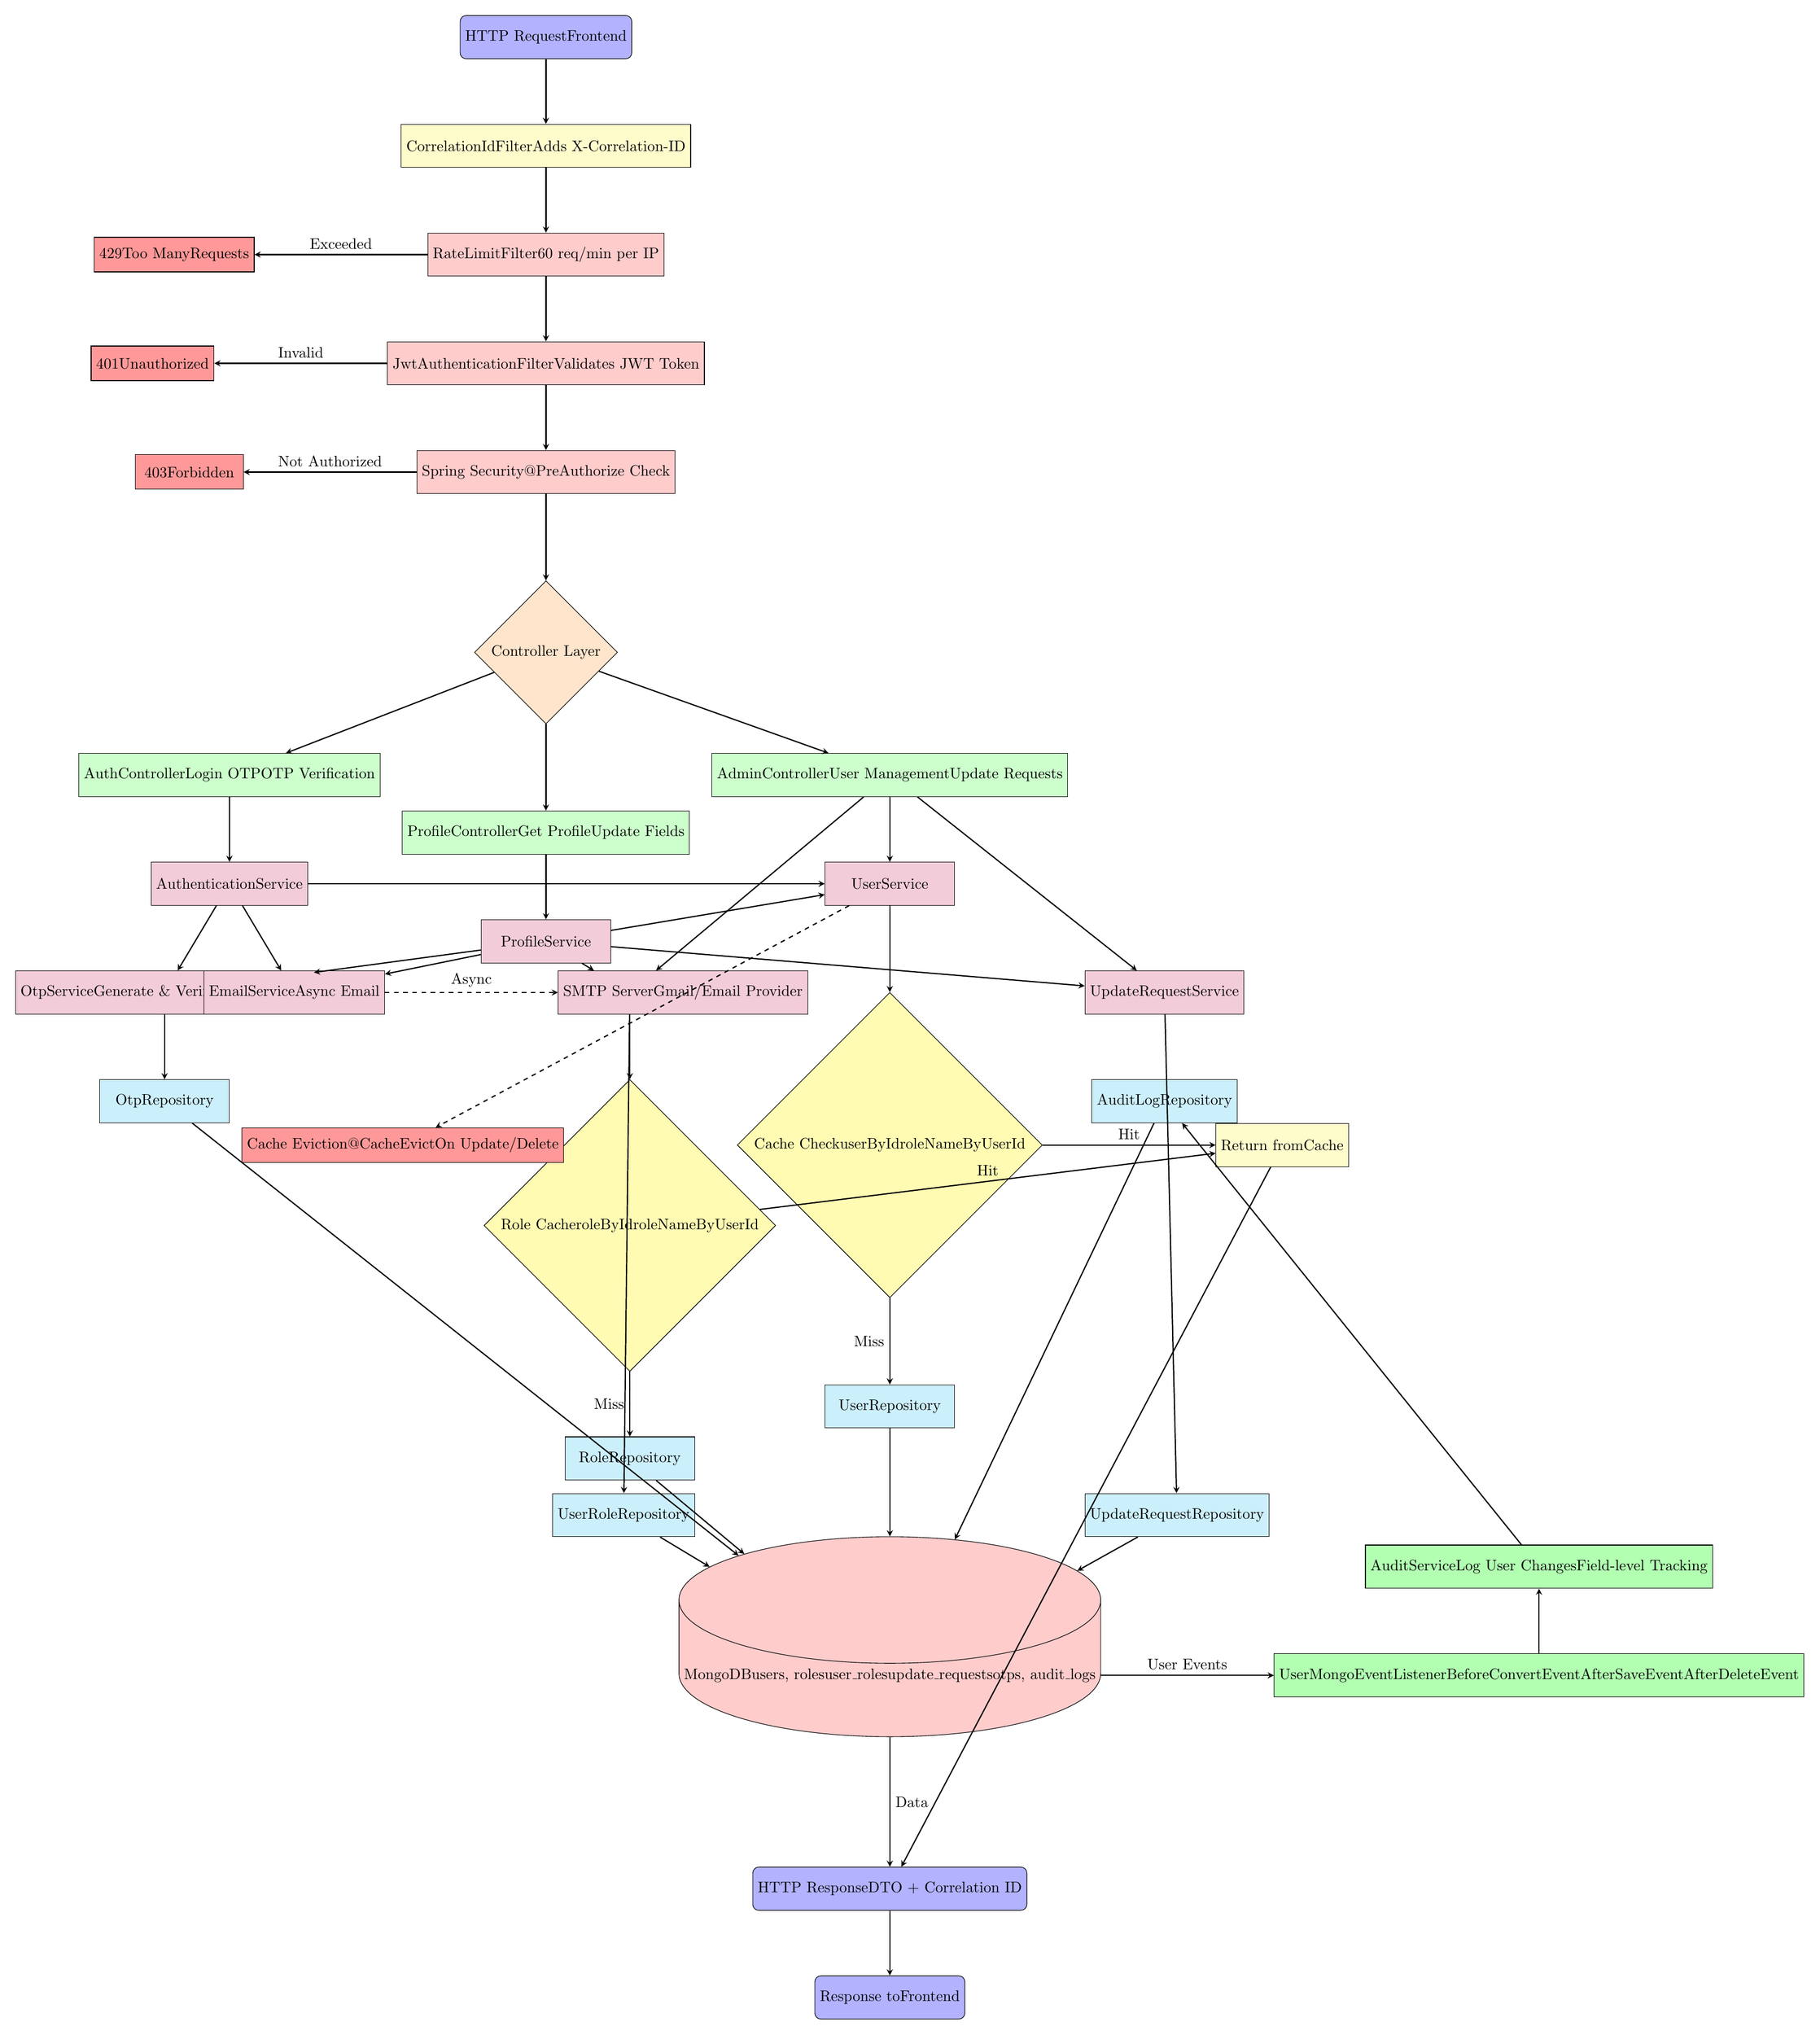
\begin{tikzpicture}[
    node distance = 1.5cm and 2cm,
    auto,
    % Styles
    startstop/.style={rectangle, rounded corners, minimum width=3cm, minimum height=1cm, text centered, draw=black, fill=blue!30},
    process/.style={rectangle, minimum width=3cm, minimum height=1cm, text centered, draw=black, fill=yellow!20},
    security/.style={rectangle, minimum width=3cm, minimum height=1cm, text centered, draw=black, fill=red!20},
    controller/.style={rectangle, minimum width=3cm, minimum height=1cm, text centered, draw=black, fill=green!20},
    service/.style={rectangle, minimum width=3cm, minimum height=1cm, text centered, draw=black, fill=purple!20},
    cache/.style={diamond, minimum width=2.5cm, minimum height=1.5cm, text centered, draw=black, fill=yellow!30},
    repository/.style={rectangle, minimum width=3cm, minimum height=1cm, text centered, draw=black, fill=cyan!20},
    database/.style={cylinder, shape border rotate=90, aspect=0.3, minimum width=3cm, minimum height=2cm, text centered, draw=black, fill=red!20},
    listener/.style={rectangle, minimum width=3cm, minimum height=1cm, text centered, draw=black, fill=green!30},
    decision/.style={diamond, minimum width=2.5cm, minimum height=1.5cm, text centered, draw=black, fill=orange!20},
    error/.style={rectangle, minimum width=2.5cm, minimum height=0.8cm, text centered, draw=black, fill=red!40},
    arrow/.style={thick,->,>=stealth}
]

% Start
\node [startstop] (start) {HTTP Request\\Frontend};

% Filters
\node [process, below=of start] (corrFilter) {CorrelationIdFilter\\Adds X-Correlation-ID};
\node [security, below=of corrFilter] (rateFilter) {RateLimitFilter\\60 req/min per IP};
\node [security, below=of rateFilter] (jwtFilter) {JwtAuthenticationFilter\\Validates JWT Token};

% Security
\node [security, below=of jwtFilter] (security) {Spring Security\\@PreAuthorize Check};

% Controllers
\node [decision, below=of security, yshift=-0.5cm] (controller) {Controller Layer};
\node [controller, below left=of controller, xshift=-1cm] (authCtrl) {AuthController\\Login OTP\\OTP Verification};
\node [controller, below=of controller, yshift=-0.5cm] (profileCtrl) {ProfileController\\Get Profile\\Update Fields};
\node [controller, below right=of controller, xshift=1cm] (adminCtrl) {AdminController\\User Management\\Update Requests};

% Services
\node [service, below=of authCtrl] (authSvc) {AuthenticationService};
\node [service, below=of profileCtrl] (profileSvc) {ProfileService};
\node [service, below=of adminCtrl] (userSvc) {UserService};
\node [service, below right=of userSvc, xshift=1cm] (updateReqSvc) {UpdateRequestService};
\node [service, below left=of userSvc, xshift=-1cm] (roleSvc) {RoleService};

% Additional Services
\node [service, below=of authSvc, xshift=-1.5cm] (otpSvc) {OtpService\\Generate \& Verify\\Rate Limiting};
\node [service, below=of authSvc, xshift=1.5cm] (emailSvc) {EmailService\\Async Email};

% Cache Checks
\node [cache, below=of userSvc, yshift=-0.5cm] (cacheCheck) {Cache Check\\userById\\roleNameByUserId};
\node [cache, below=of roleSvc] (roleCache) {Role Cache\\roleById\\roleNameByUserId};

% Repositories
\node [repository, below=of cacheCheck, yshift=-0.5cm] (userRepo) {UserRepository};
\node [repository, below=of roleCache] (roleRepo) {RoleRepository};
\node [repository, below left=of userRepo, xshift=-1cm] (userRoleRepo) {UserRoleRepository};
\node [repository, below right=of userRepo, xshift=1cm] (updateReqRepo) {UpdateRequestRepository};
\node [repository, below=of otpSvc] (otpRepo) {OtpRepository};
\node [repository, below=of updateReqSvc] (auditRepo) {AuditLogRepository};

% Database
\node [database, below=of userRepo, yshift=-1cm] (mongodb) {MongoDB\\users, roles\\user\_roles\\update\_requests\\otps, audit\_logs};

% Event Listener
\node [listener, right=of mongodb, xshift=2cm] (eventListener) {UserMongoEventListener\\BeforeConvertEvent\\AfterSaveEvent\\AfterDeleteEvent};

% Audit Service
\node [listener, above=of eventListener] (auditSvc) {AuditService\\Log User Changes\\Field-level Tracking};

% SMTP
\node [service, right=of emailSvc, xshift=2cm] (smtp) {SMTP Server\\Gmail/Email Provider};

% Cache Operations
\node [error, left=of cacheCheck, xshift=-2cm] (cacheEvict) {Cache Eviction\\@CacheEvict\\On Update/Delete};
\node [process, right=of cacheCheck, xshift=2cm] (cacheReturn) {Return from\\Cache};

% Response
\node [startstop, below=of mongodb, yshift=-1.5cm] (response) {HTTP Response\\DTO + Correlation ID};
\node [startstop, below=of response] (end) {Response to\\Frontend};

% Error Nodes
\node [error, left=of rateFilter, xshift=-2cm] (rateError) {429\\Too Many\\Requests};
\node [error, left=of jwtFilter, xshift=-2cm] (authError) {401\\Unauthorized};
\node [error, left=of security, xshift=-2cm] (authzError) {403\\Forbidden};

% Arrows - Main Flow
\draw [arrow] (start) -- (corrFilter);
\draw [arrow] (corrFilter) -- (rateFilter);
\draw [arrow] (rateFilter) -- (jwtFilter);
\draw [arrow] (jwtFilter) -- (security);
\draw [arrow] (security) -- (controller);

% Controller to Services
\draw [arrow] (controller) -- (authCtrl);
\draw [arrow] (controller) -- (profileCtrl);
\draw [arrow] (controller) -- (adminCtrl);
\draw [arrow] (authCtrl) -- (authSvc);
\draw [arrow] (profileCtrl) -- (profileSvc);
\draw [arrow] (adminCtrl) -- (userSvc);
\draw [arrow] (adminCtrl) -- (updateReqSvc);
\draw [arrow] (adminCtrl) -- (roleSvc);

% Service Connections
\draw [arrow] (authSvc) -- (otpSvc);
\draw [arrow] (authSvc) -- (emailSvc);
\draw [arrow] (authSvc) -- (userSvc);
\draw [arrow] (profileSvc) -- (userSvc);
\draw [arrow] (profileSvc) -- (updateReqSvc);
\draw [arrow] (profileSvc) -- (otpSvc);
\draw [arrow] (profileSvc) -- (emailSvc);
\draw [arrow] (profileSvc) -- (roleSvc);
\draw [arrow] (roleSvc) -- (userRoleRepo);

% Cache Flow
\draw [arrow] (userSvc) -- (cacheCheck);
\draw [arrow] (cacheCheck) -- node[left] {Miss} (userRepo);
\draw [arrow] (cacheCheck) -- node[above] {Hit} (cacheReturn);
\draw [arrow] (roleSvc) -- (roleCache);
\draw [arrow] (roleCache) -- node[left] {Miss} (roleRepo);
\draw [arrow] (roleCache) -- node[above] {Hit} (cacheReturn);

% Repository to Database
\draw [arrow] (userRepo) -- (mongodb);
\draw [arrow] (roleRepo) -- (mongodb);
\draw [arrow] (userRoleRepo) -- (mongodb);
\draw [arrow] (updateReqRepo) -- (mongodb);
\draw [arrow] (otpRepo) -- (mongodb);
\draw [arrow] (updateReqSvc) -- (updateReqRepo);
\draw [arrow] (otpSvc) -- (otpRepo);

% Event Listener Flow
\draw [arrow] (mongodb) -- node[above] {User Events} (eventListener);
\draw [arrow] (eventListener) -- (auditSvc);
\draw [arrow] (auditSvc) -- (auditRepo);
\draw [arrow] (auditRepo) -- (mongodb);

% Cache Eviction
\draw [arrow, dashed] (userSvc) -- (cacheEvict);

% Email Flow
\draw [arrow, dashed] (emailSvc) -- node[above] {Async} (smtp);

% Response Flow
\draw [arrow] (cacheReturn) -- (response);
\draw [arrow] (mongodb) -- node[right] {Data} (response);
\draw [arrow] (response) -- (end);

% Error Flows
\draw [arrow] (rateFilter) -- node[above] {Exceeded} (rateError);
\draw [arrow] (jwtFilter) -- node[above] {Invalid} (authError);
\draw [arrow] (security) -- node[above] {Not Authorized} (authzError);

\end{tikzpicture}
\end{document}


